\documentclass[lettersize,journal]{IEEEtran}
\usepackage{amsmath,amsfonts}
\usepackage{algorithmic}
\usepackage{algorithm}
\usepackage{array}
\usepackage{minted}
\usepackage[caption=false,font=normalsize,labelfont=sf,textfont=sf]{subfig}
\usepackage{textcomp}
\usepackage{lipsum}
\usepackage[export]{adjustbox}
\usepackage{stfloats}
\usepackage{url}
\usepackage{verbatim}
\usepackage{graphicx}
\usepackage{cite}
\usepackage{hyperref}
\usepackage{enumitem}
\usepackage{listings}
 \usepackage{booktabs}
\hyphenation{op-tical net-works semi-conduc-tor IEEE-Xplore}
% updated with editorial comments 8/9/2021
\usepackage{utfsym}
\usepackage{makecell}
\def\checkmark{\usym{1F5F8}} 
\newcommand{\cfgfiles}{configuration files}
\newcommand{\cfgfile}{configuration file}


\begin{document}

\title{Design, Implementation, and Evaluation of a Meta Configuration Tool Using Schema-to-UI Approaches}
\author{Felix Neubauer, Paul Bredl, Minye Xu, Keyuriben Patel}
%\author{IEEE Publication Technology,~\IEEEmembership{Staff,~IEEE,}
        % <-this % stops a space
%\thanks{This paper was produced by the IEEE Publication Technology Group. They are in Piscataway, NJ.}% <-this % stops a space
%\thanks{Manuscript received April 19, 2021; revised August 16, 2021.}}

% The paper headers
\markboth{Journal of best software 2023}%
{Shell \MakeLowercase{\textit{et al.}}: Revolutionizing Software}

%\IEEEpubid{0000--0000/00\$00.00~\copyright~2021 IEEE}
% Remember, if you use this you must call \IEEEpubidadjcol in the second
% column for its text to clear the IEEEpubid mark.

\maketitle

\begin{abstract}
This document describes the most common article elements and how to use the IEEEtran class with \LaTeX \ to produce files that are suitable for submission to the IEEE.  IEEEtran can produce conference, journal, and technical note (correspondence) papers with a suitable choice of class options. 
\end{abstract}

\begin{IEEEkeywords}
Article submission, IEEE, IEEEtran, journal, \LaTeX, paper, template, typesetting.
\end{IEEEkeywords}

\section{Introduction} %felix

Textual formats to structure data, such as JSON, XML and YAML, are human readable as well as machine readable.

For configuration files such formats are often used, since they can be read and maintained by humans, as well as deserialized and used by computer programs. 
The format of those data structures can be defined by so-called schemas, which define the rules the data has to conform to.
Besides configuration files and the field of software development, other academic fields, such as Biology or Chemistry also use those formats to structure and validate their data.

To simplify, we will call all file instances using such formats \textit{\cfgfiles}.

Depending on the content of such \cfgfiles, they can be complex and time-consuming to modify and maintain. 
Tooling, such as graphical user interfaces, can significantly reduce manual efforts and assist the user. 
Those graphical user interfaces, however, require initial effort to be developed, as well as continuous effort in being maintained and updated when the underlying configuration schema changes. 
We intend to tackle this problem by developing a meta program that allows humans to generate such configurator GUIs, which can be shared with others.

Our approach differs from other schema-to-UI approaches in following:

\begin{enumerate}
    \item The tool combines the assistance of a GUI with the flexibility and speed of a rich-text editor by providing both in one view
    \item The schema can be defined using the same tool
    \item The defined schemas, the resulting configurator GUI and the modified configuration files can all be shared with others
\end{enumerate}


In section~\ref{sec:research} we will introduce related work and introduce existing schema formats as well as schema-to-gui approaches.
Next we will discuss the design of our solution (section TODO).



% Summary of our approach/idea and reference the different sections, e.g. in Section 1 we will research existing work on that area and then in section 2 blabla.

\section{Related Work}\label{sec:research} % intro: felix

This sections covers existing approaches to handle \cfgfiles{} as well as existing schema languages. We compare them briefly and discuss why JSON schema is the most useful language for our approach. As our research is of practical nature, we also consider gray literature like specifications of schemas or websites.

\subsection{Existing Approaches}
% felix
There exist several approaches that attempt to make maintaining \cfgfiles{} easier for the user. Most of these approaches depend on the schema of the configuration file to be known. Based on such a schema, it is possible to validate whether the config file adheres to the schema. Findings from such a schema validation can be shown to the user, for example via syntax highlighting. Additionally, the user can be assisted by means of graphical user interfaces.

% minye
\begin{listing}[!h]
\begin{minted}[frame=single,
               framesep=3mm,
               linenos=true,
               xleftmargin=15pt,
               tabsize=4]{js}
{
  "$id": "https://example.com
  /person.schema.json",
  "$schema": "https://json-schema.org
  /draft/2020-12/schema",
  "title": "Person",
  "type": "object",
  "properties": {
    "firstName": {
      "type": "string",
      "description": "first name."
    },
    "lastName": {
      "type": "string",
      "description": "last name."
    },
    "age": {
      "description": "Age",
      "type": "integer",
      "minimum": 0
    }
  }
}
\end{minted}
\caption{JSON schema example} 
\label{json-schema-example}
\end{listing}


\begin{listing}[!h]
\begin{minted}[frame=single,
               framesep=3mm,
               linenos=true,
               xleftmargin=15pt,
               tabsize=4]{js}
{
  "firstName": "John",
  "lastName": "Doe",
  "age": 21
}
\end{minted}
\caption{JSON example for the schema shown in Listing \ref{json-schema-example}} 
\label{json-example}
\end{listing}


\subsubsection{Schema Validation} % Keyuri
Schema validation is the process of checking whether a given data instance (e.g., a JSON, YAML or XML document) conforms to a predefined schema. The specification for JSON schema validation can be found in the work of \cite{JSON_schema_vailidation} \cite{JSONValidation}. Listing \ref{json-schema-example} is an exemplary JSON schema. It could be used to validate the example instance shown in Listing \ref{json-example}.
%We can also use a python library to validate.\ref{python_json_validation}

% \begin{figure}[!t]
% \centering
% 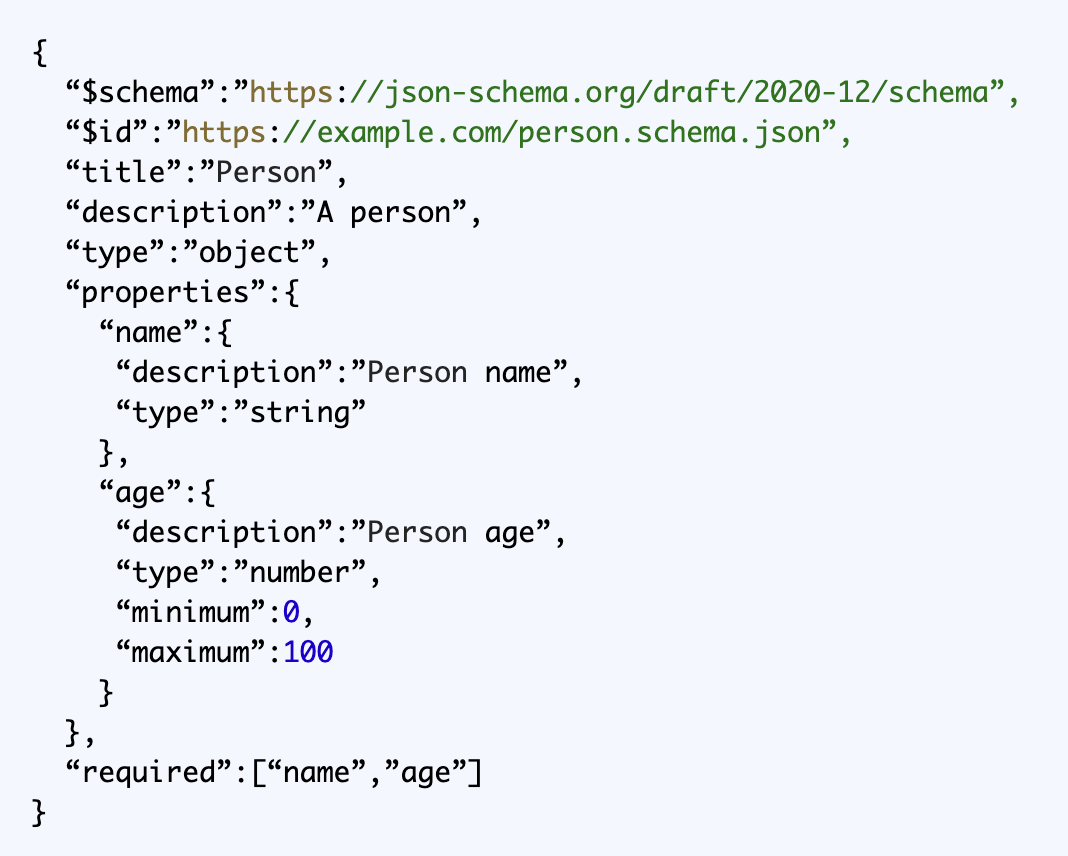
\includegraphics[width=2.5in]{schema_validation_demo.jpg}
% \caption{JSON schema demo}
% \label{schema_validation_demo}
% \end{figure}



% \begin{figure}[!t]
% \centering
% 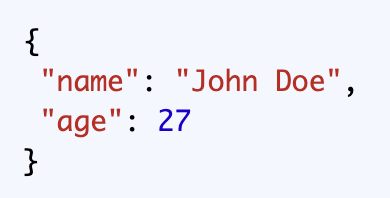
\includegraphics[width=2.5in]{instance_demo.jpg}
% \caption{Instance for validation}
% \label{instance_demo}
% \end{figure}

% \begin{figure}[!t]
% \centering
% 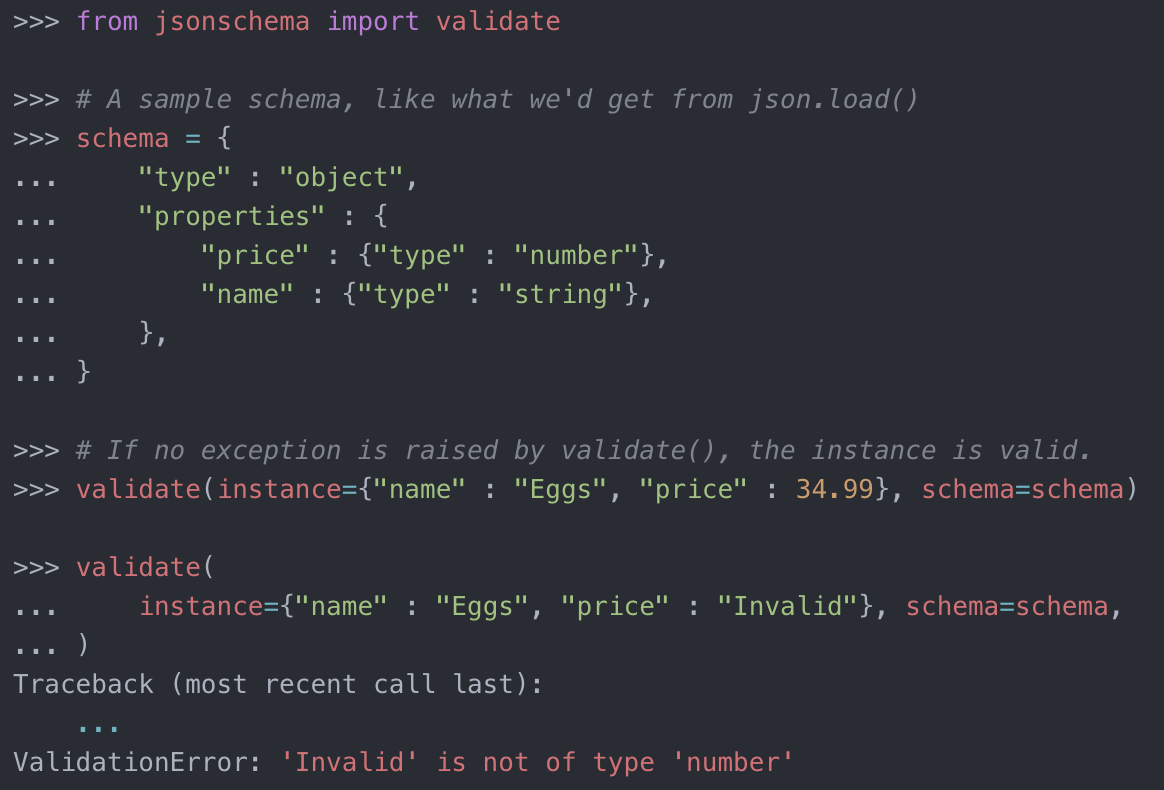
\includegraphics[width=2.5in]{python_json_validation.png}
% \caption{Validation using python library}
% \label{python_json_validation}
% \end{figure}

% todo: add paper about schema validation and possibly a small example

\subsubsection{Schema to GUI}
% minye and felix
Refers to the process of generating a graphical user interface (GUI) based on a predefined schema. Such GUIs can assist the user in a multitude of ways, such as help by tooltips (Figure \ref{gui_advantage_tooltip}), Auto-Completion (Figure \ref{gui_advantage_autocomplete}) and Choice Selections (Figure \ref{gui_advantage_choiceselection}).

\begin{figure}[!t]
\centering

\includegraphics[width=2.5in]{gui_advantage_tooltip.png}
\caption{Tooltip Assistance}
\label{gui_advantage_tooltip}
\end{figure}

\begin{figure}[!t]
\centering
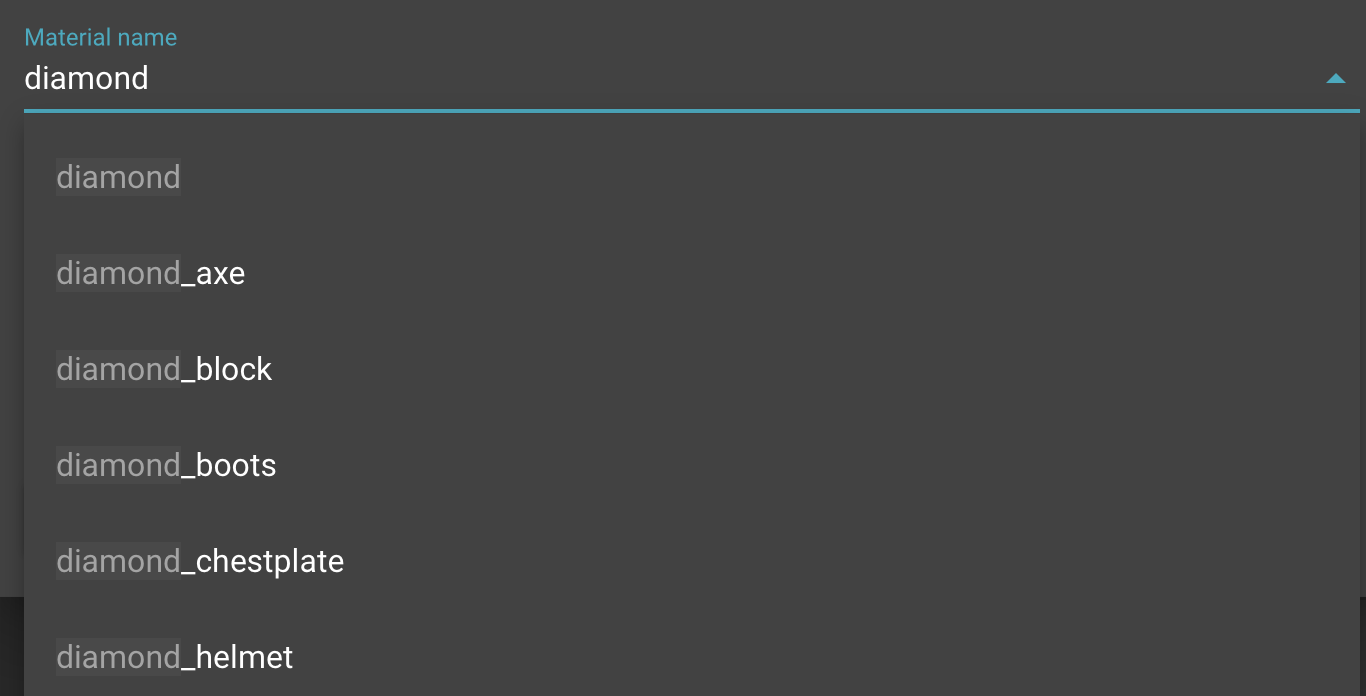
\includegraphics[width=2.5in]{gui_advantage_autocomplete.png}
\caption{Auto-Completion}
\label{gui_advantage_autocomplete}
\end{figure}

\begin{figure}[!t]
\centering
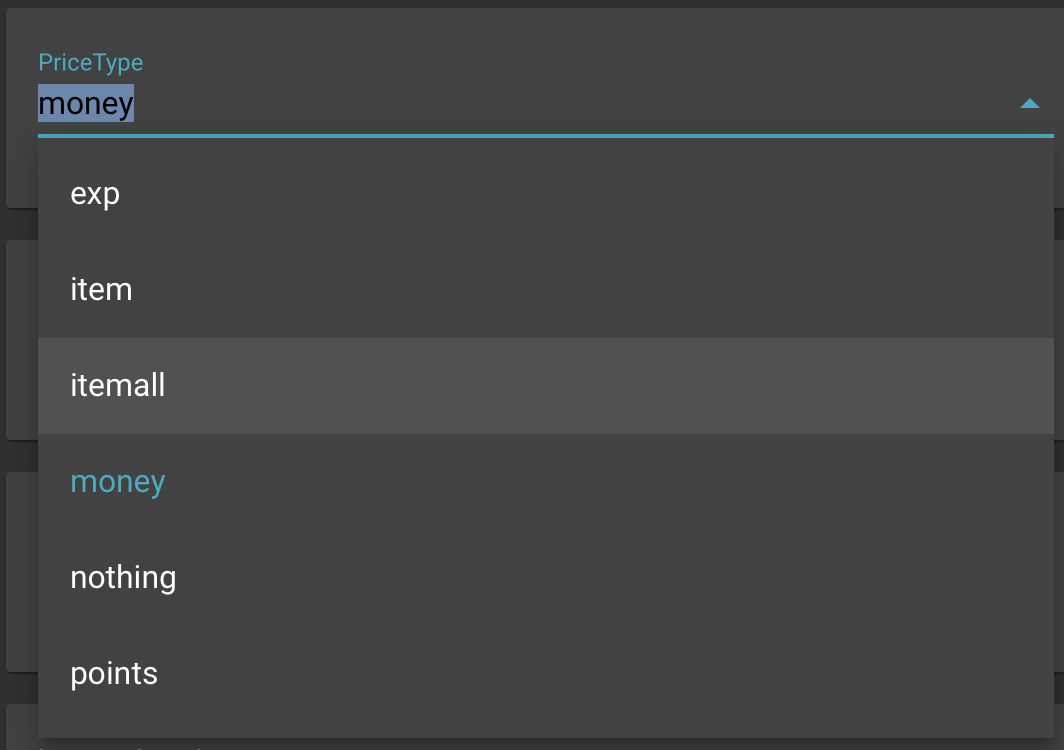
\includegraphics[width=2.5in]{gui_advantage_choiceselection.png}
\caption{Choice Selection}
\label{gui_advantage_choiceselection}
\end{figure}

% felix
By inherently adhering to the schema structure, with such GUIs configuration errors are avoided or at least significantly reduced. Users not very familiar with the configuration schema profit most from the GUI assistance, but even experienced users tend to not remember every individual detail of the schema and benefit.

In the following, existing schema-to-UI approaches are listed.


% Minye
\begin{enumerate}[label=(\alph*)]
    \item \textbf{Vue Form Generator}\cite{vueformgenerator}: is a schema-based form generator component for Vue.js. It can be extended with custom fields. At the time of writing this paper the tool was rated with most stars among web form generator projects.
    
    \item \textbf{JSON Forms} \cite{JSONForms}: is a declarative framework for building form-based web UIs. It can be integrated with UI libraries or frameworks, such as Vue, React or Angular.
    
    \item \textbf{Adamant}\cite{siffa2022adamant}: also is a JSON-schema based form generator, that supports any valid schema. It also supports schema validation.
    
\end{enumerate}

% paul
\subsection{Schema Languages}\label{sub:schemalanguages}

Schema languages are formal languages that specify the structure, constraints, and relationships of data, for example in a database or in structured data formats. Schema languages are text based, we do not consider any graphical modeling languages like UML.

For this work we consider using an existing schema language (or a subset of it), building on an existing schema language or introducing our own schema language.
The following sections describe existing schema languages.

%paul
\subsubsection{JSON schema}

JSON is a common data-interchange format for exchanging data with webservices, but also for storing documents in noSQL databases like MongoDB.
Because of the popularity of JSON, a demand for a schema for JSON documents evolved, which resulted in JSON schema \cite{jsonSchema, jsonschemaJSONSchema}. 

JSON schema has evolved to being the de-facto standard schema language for JSON documents. Schemas for many popular \cfgfile{} types exist. JSON schema store\footnote{\url{https://www.schemastore.org/json/}} is a website that lists at the time of access 669 file types, for which they provide a JSON schema file. The supported file types include for example Docker compose or OpenAPI files. \cite{barbaglia, ChaeronySiffa2022} give further examples of JSON schema used in practice. 


JSON and YAML documents are of a similar structure (JSON being a subset of YAML) and JSON schema can be applied on YAML documents too. Some syntactical details of YAML can, however, not be expressed with JSON schema. 

% felix
\subsubsection{XSD and DTD}
For XML the two de-facto standard schema languages are Document Type Definition (DTD)\cite{dtd_spec} and XML Schema Definition (XSD)\cite{xsd_spec}. 
XSD is the newer and more expressive format of them and in large parts replaces and supersedes the more limited format DTD\cite{dtd_vs_xsd}. 
It is recommended by W3C\cite{xsd_spec}. 

Multiple more schema languages have been proposed and developed but are relatively unknown compared to XSD\cite{xml_schemas_1}\cite{xml_schemas_2}.

\subsubsection{CUE}\cite{cuelang} %Minye
(Configure, Unify, Execute) is a data validation and configuration language, which can be used with various data formats, such as JSON and YAML (it is a superset of both).
It has several use cases, especially in configuration and data validation.


\subsubsection{Apache Avro}% Keyuri
is an open source project that provides data serialization and data exchange services for Apache Hadoop.
It uses a JSON-based schema language~\cite{Apache-Avro}.

% TODO: reference to specs/website

% paul
\subsubsection{Other formats}

There exist other formats for defining data structures. We also evaluated the GraphQL schema language and protobuf (also known as Protocol Buffers)
%protocol buffer?
The GraphQL schema language is used to define the data structures of GraphQL APIs~\cite{graphQL}. Protobuf is a language for data serialization by Google~\cite{protobufProtocolBuffers}.

% Paul
\subsection{Evaluation of Schema Languages}

% Support for Reference


We evaluate several schema languages in how well they fit our use-case. Ideally, the schema language is both popular and supported by numerous tools and libraries and expressive in a sense that id provides metadata that can be used to display in the GUI editor to assist the user. 

\subsubsection{Evaluation criteria} % evaluation by paul, some criteria ideas by felix

We evaluated the seven schema languages we mentioned in section~\ref{sub:schemalanguages} based on the following criteria and metrics:
\begin{enumerate}
% metric: Stackoverflow question # with schema language as tag
    \item \textbf{Practical usage} --- Ideally our approach uses a schema language that already known by many developers. 
    As indicator of the practical usage we use the approximate search results on stackoverflow.com as metric. 
    We aquire the results by querying the google search engine with the name of the schema language and "site:stackoverflow.com", which limits the search results to stackoverflow.com. 
    This metric might also correlate with the complexity of the schema language as a more complex to use schema language will likely lead to more questions asked on the site. Nevertheless, we assume that a significantly higher number of results indicates that a language is more known than others.

    Additionally, we investigate how well the schema languages are supported by IDEs and code libraries.
    \begin{enumerate}
        \item \textit{Tool support} --- We used the 10 most popular IDEs\cite{mostpopularides} and checked if the IDE supports the schema language either natively or by a plugin. Support here means that either the IDE is capable of validating documents against a schema in the schema language or supports creating schema files, e.g. by using syntax highlighting for the schema language.
        % # node modules with schema language keyword....
        \item \textit{Library support} --- As we implement a web-based tool, we JavaScript or TypeScript bases tools are helpful for our approach, e.g. so we can reuse a package for schema validation. We investigate the number of node modules exist that are related to the schema languages by querying the node module search on \url{www.npmjs.com} with the name of the schema language.
        
    \end{enumerate}

    % # of cases fulfilled from below
    \item \textbf{Expressiveness} --- We evaluate how expressive each of the schema languages are, i.e. what possible constructs the language is able to express. We defines eight requirements on the language features that we consider helpful for our approach. The number of requirements a schema language fulfills is our metric that indicates how expressive the language is. Table~\ref{tab:comparison} reports the results. The eight requirements are:
    \begin{enumerate}
        \item \textit{Simple types} --- This is fulfilled if the schema language provides the possibility to define simple data types, at least strings, numeric types, and a boolean type. This is a fundamental feature required for our approach.
        \item \textit{Complex types} --- This is fulfilled if the schema language provides the possibility to define complex data types, at least records and arrays.
        This is crucial feature for our approach as configuration files are often structured data rather than plain key-value pairs.
        \item \textit{Descriptions} --- This is fulfilled if the schema language provides the possibility to add descriptions to fields. This is helpful in a schema-to-GUI approach as the description can be shown to the user, providing potential helpful information on how a field should be filled.
        \item \textit{Examples} --- This is fulfilled if the schema language provides the possibility to add example values. This is helpful in our approach as the example values can serve as placeholders in the GUI editor.
        \item \textit{Default values} --- This is fulfilled if the schema language provides the possibility to add default values which are assumed in an absence of a value. This often helpful information can be displayed to the user or used as placeholder values.
        \item \textit{Optional values} --- This is fulfilled if the schema language provides the possibility to declare values as optional or required. Often it is not necessary to provide all values in a configuration file, so it is helpful to mark fields as required or optional in the GUI editor.
        \item \textit{Constraints} --- This is fulfilled if the schema language provides the possibility possibility to constrain values of fields, e.g. maximum length of strings. To be exact, for this evaluation we required that at least two of the following constrained can be expressed by the schema language:
        \begin{itemize}
            \item The length of strings can be limited.
            \item The range of numeric types can be limited, e.g. to only positive values.
            \item The valid values of a field can be restricted to a finite amount of values (enumeration).
            \item The format of a string field can be constrained to a certain pattern.
        \end{itemize}
        This is a helpful feature for our approach as often not all possible values are valid for specific fields in configuration files.
        \item \textit{Conditions} --- This is fulfilled if the schema language provides the possibility to define conditional dependencies between fields. This is a advanced feature that is helpful because it allows to express for example that a particular field must be given only if another field has a specific value.
        \item \textit{References} --- This is fulfilled if the schema language provides the possibility to define reusable subschemas that can be referenced in other parts of the schema. This is often useful in practice to reuse common data structures.
    \end{enumerate}
    
    %\item \textbf{Support for XML, YAML, or JSON} ---  
    
    % For our approach we aim to use the same or at least a very similar editor for both editing the actual \cfgfiles and the schema files. Consequently, the schema language should be a subset of the language that the \cfgfiles are written in, i.e. the document language. For example JSON schema files are JSON files and JSON schema is used to validate JSON files, so here this criteria is fulfilled. In constrast, DTD is a schema language for validating XML files but a DTD file is not a valid XML file.
    
\end{enumerate}

    
    \begin{table*}[]
    \centering
    \caption{Evaluation of different schema languages\label{tab:all}}
        \begin{tabular}{@{}lrrrr@{}}
        \toprule
        \textbf{Schema language} &
          \textbf{\# Search results } &
          \textbf{IDE support} &
          \textbf{\# Node packages} &
          \textbf{Expressiveness} \\ \midrule
        JSON schema &
          245.000 &
          8 / 10 &
          4.536 & 8 / 8  \\
        XSD & 151.000 & 8 / 10 & 116 & 7 / 8 \\
        DTD & 69.700 & 9 / 10 & 34 & 5 / 8\\
        CUE & 10.500 & 4 / 10 & 97 & 7 / 8 \\
        Avro & 20.000 & 8 / 10 & 211 & 4 / 8 \\
        protobuf &  44.800 & 9 / 10 & 1.210 & 3 / 8\\
        GraphQl schema & 31.000 & 7 / 10 & 1.509 & 5 / 8\\ \bottomrule
        \end{tabular}
    \end{table*}
    %\label{fig:my_label}
%\end{figure}

% IDE                | JSON schema | XSD | DTD | CUE | Avro | protobuf | GraphQL schema |
% Visual Studio      | yes         | yes | yes | x   | yes  | yes      | yes            |
% Visual Studio Code | yes         | yes | yes | yes | yes  | yes      | yes            |
% Eclipse            | yes         | yes | yes | x   | yes  | yes      | x              |
% pyCharm            | yes         | yes | yes | yes | yes  | yes      | yes            |
% Android Studio     | yes         | yes | yes | yes | yes  | yes      | yes            |
% IntelliJ           | yes         | yes | yes | yes | yes  | yes      | yes            |
% NetBeans           | x           | yes | yes | x   | x    | yes      | x              |
% RStudio            | x           | x   | x   | x   | x    | x        | x              |
% Atom               | yes         | x   | yes | x   | yes  | yes      | yes            |
% Sumblime Text      | yes         | yes | yes | x   | yes  | yes      | yes            |
% ======================================================================================|
%                    | 8 / 10      | 8   | 9   | 4   | 8    | 9        | 7              |

\begin{table*}
    \centering
    \caption{Comparison of expressiveness of different schema languages
    \label{tab:comparison}}
    \begin{tabular}{@{}lllllllllr@{}}
         \toprule
        \textbf{Schema language} &
          \thead{Simple \\ types} &
          \thead{Complex \\ types} &
          \thead{Descriptions} &
          \thead{Example \\ values} &
          \thead{Default \\ values} &
          \thead{Optional \\ values} &
          \thead{Constraints} &
          \thead{Conditions}  &
          \thead{Result}\\ \midrule
        JSON schema &
          \checkmark &
          \checkmark &
          \checkmark &
          \checkmark &
          \checkmark &
          \checkmark &
          \checkmark &
          \checkmark & 8 / 8\\ 
        XSD &
          \checkmark &
          \checkmark &
          \checkmark &
          x &
          \checkmark &
          \checkmark &
          \checkmark &
          \checkmark\footnote{using assertions}& 7 / 8 \\
        DTD &
         \checkmark &
         \checkmark &
         x &
         x &
         \checkmark &
         \checkmark &
         x &
         \checkmark & 5 / 8\\
        CUE &
         \checkmark &
         \checkmark &
         \checkmark &
         (\checkmark)\footnote{only comments} &
         x &
         \checkmark &
         \checkmark &
         \checkmark & 7 / 8\\
        Avro &
         \checkmark &
         \checkmark &
         x &
         x & 
         \checkmark &
         \checkmark \footnote{Only allowing nullability, no distinction to absent values} &
         x &
         x & 4 / 8\\
        protobuf &
            \checkmark &
            \checkmark &
            x &
            x &
            x &
            \checkmark &
            x &
            x& 3 / 8 \\
        GraphQL schema &
         \checkmark &
         \checkmark &
         \checkmark &
         x &
         \checkmark &
         \checkmark &
         x &
         x & 5 / 8\\
          \bottomrule
    \end{tabular}
\end{table*}

% paul
\subsubsection{Evaluation results}

Table~\ref{tab:all} shows the results of our evaluation. We come to the conclusion that JSON schema is sufficiently popular and expressive that we choose to use it as the schema language for our approach.

% paul
\subsection{JSON schema versions}

JSON schema has had 10 different drafts over the years, the newest being draft 2020-12~\cite{jsonschemaJSONSchema}. In real-world schemas we cannot expect schemas to all have the newest version. Baazizi et al.~\cite{baazizi2021empirical} investigated over 82.000 open-source schemas in 2021, where they found that most of the are using draft 4, which was released in 2013. As the different drafts are not necessarily compatible with each other, we need to support different drafts. However, Viotto et al.~\cite{Viotti_Lagoni_2023} provide a library for migration schemas from older versions to the newest draft without loss of information. Thus, our tool only needs to support the newest draft directly. If a user uses a schema from an older draft, we first migrate it to the newest draft internally.

% paul
\subsection{Schema inference}

Schema inference is the process of deriving a schema from existing data. For our use case, this means inferring JSON schema from JSON documents. 
Frozza et al.~\cite{8424731} and Klettke et al.~\cite{klettke} present algorithms for JSON schema inference from JSON data of NoSQL data storages. Baazizi et al.\cite{Baazizi2019} also investigate schema inference from massive data sets but their approach uses its own type system rather than JSON schema.

In our tool we only aim to infer a schema from a single sample, as an optional assisting feature for our users, for which various libraries exist~\cite{githubGitHubJsonsystemspublic, githubGitHubSaasquatchjsonschemainferrer, probst_siegel_2023}.




\section{Design}

% TODO: explain why and how we define our own meta schema based on json schema, because we use just subset of its features and because our schema is used to generate schema editor GUI and therefore should only show what is supported. Also we want to add descriptions and maybe more. Also limit options to not overwhelm and confuse the user. 



% felix
\subsection{Functionality}
Before we dive into the architecture and detailed design of the tool, this section sketches what functionality the tool should have, from the viewpoint of a user.

Figure \ref{mockup_gui_config} shows how the tool could look like for the user. 


\begin{figure*}[!t]
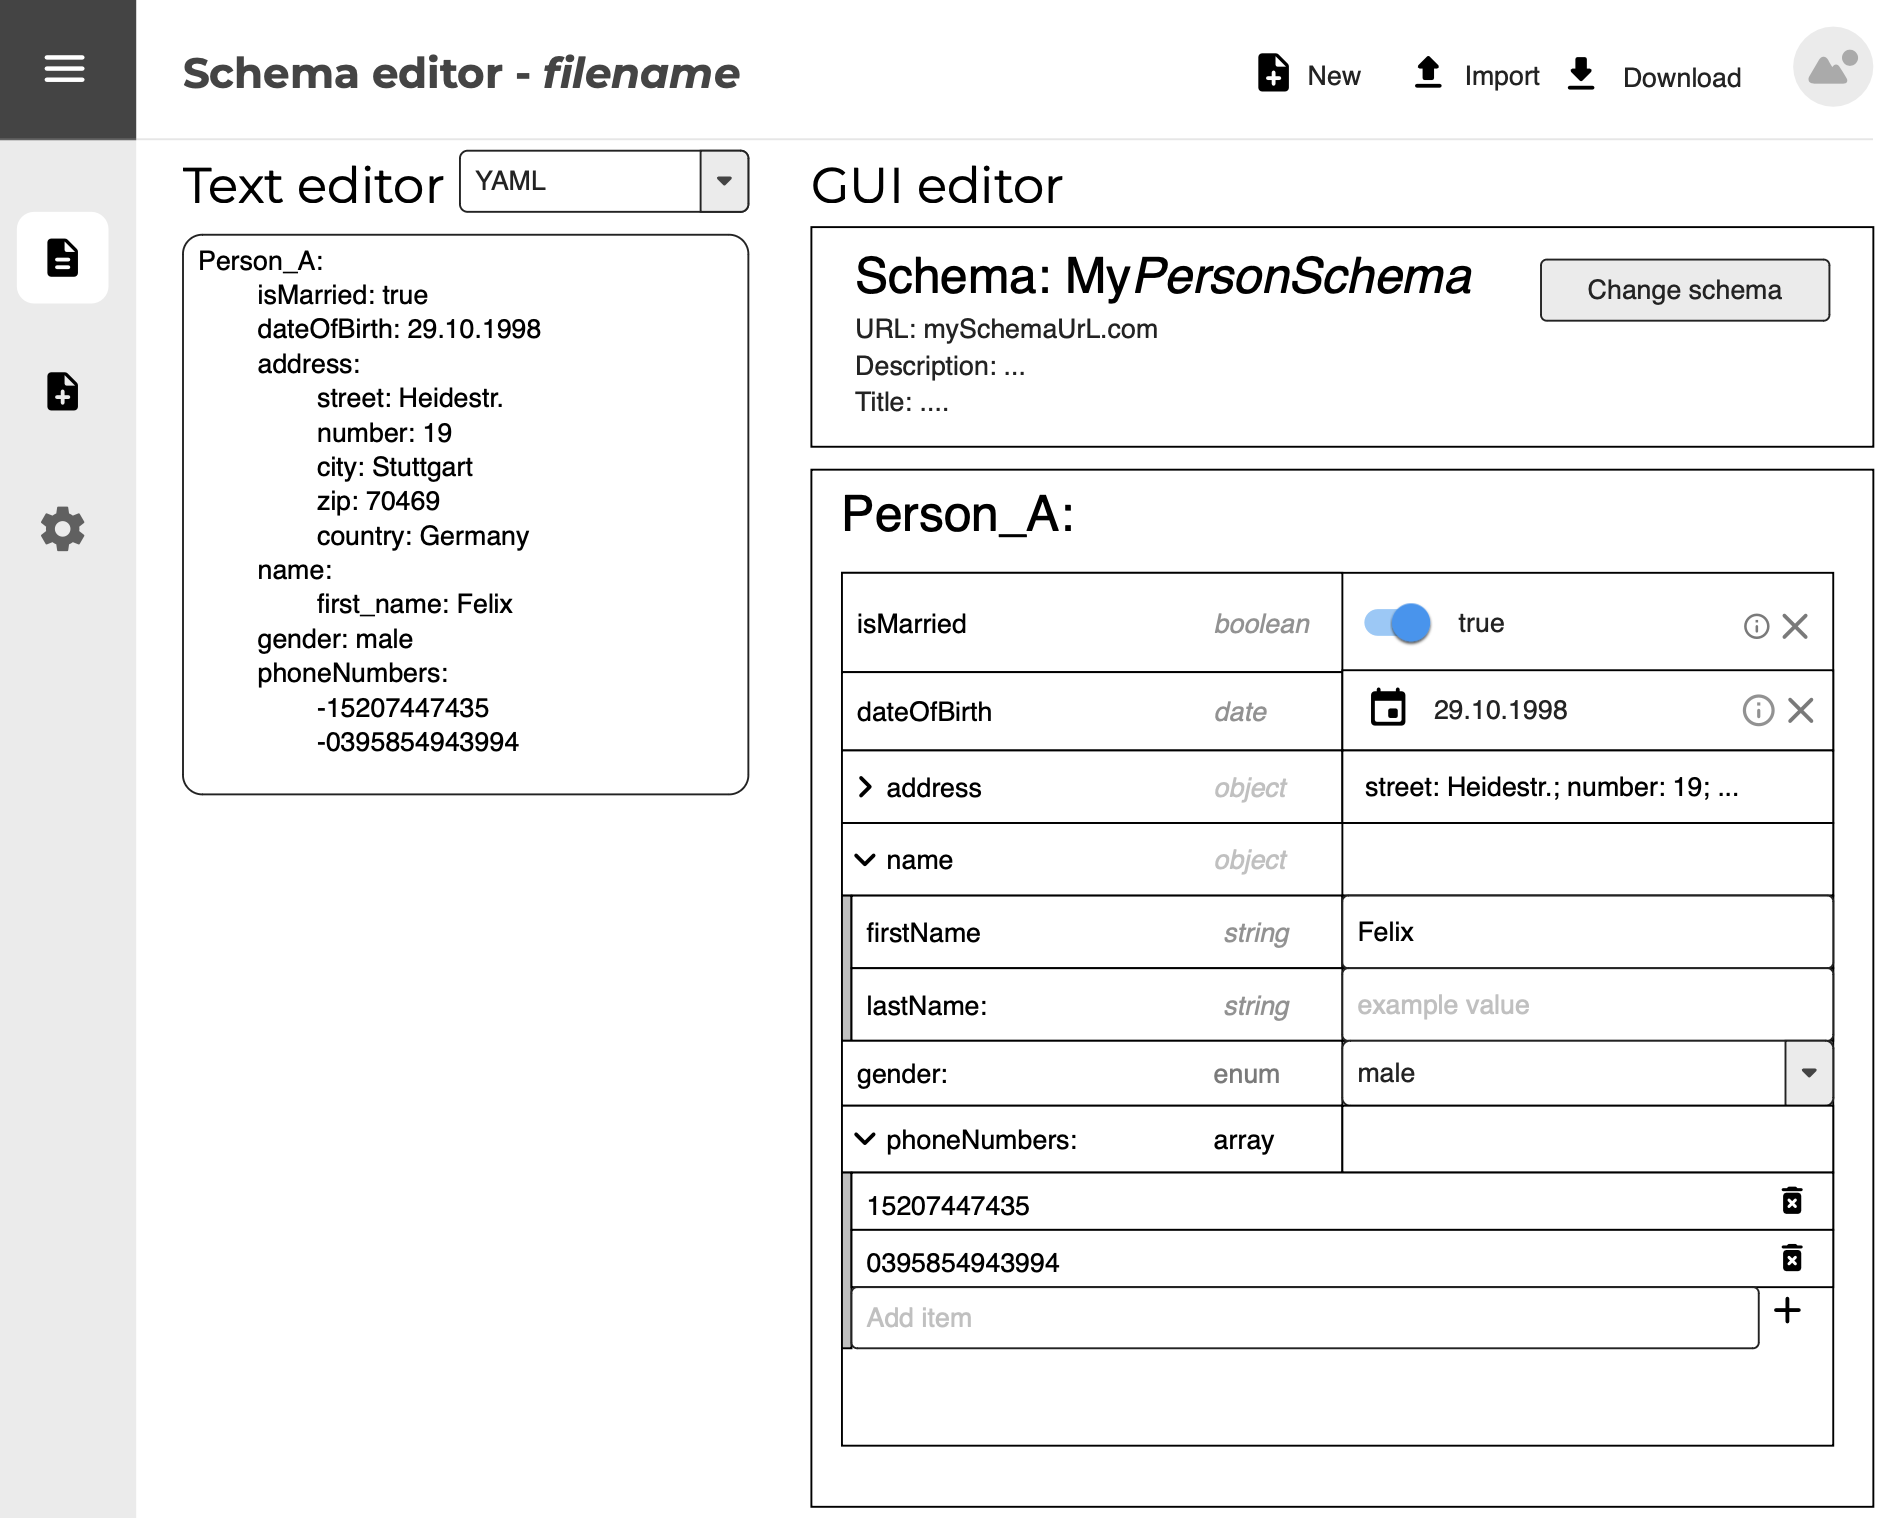
\includegraphics[width=\textwidth]{mockup_gui_config.png}
\caption{Sketch of the Tool. Workflow: the user edits their use-case specific config file based on their use-case specific schema}
\label{mockup_gui_config}
\end{figure*}

% TODO: add numbered annotations to the screenshot and explain them here
\begin{enumerate}
    \item Blabla this is the menu bar
\end{enumerate}


Besides the workflow of editing a config file, the user can also use the tool to create a new use-case specific schema. This is illustrated in figure \ref{mockup_gui_schema}. The schema called \textit{MyPersonSchema} that was used in figure \ref{mockup_gui_config} is being defined in figure \ref{mockup_gui_schema}. As a schema is a \cfgfile{} itself, it can be treated as such and the tool can offer assistance accordingly. Note that whenever the user edits a \cfgfile{} using the tool, they do so using some underlying schema. When editing a schema file, the underlying schema will be the schema of JSON Schema.

\begin{figure*}[!t]
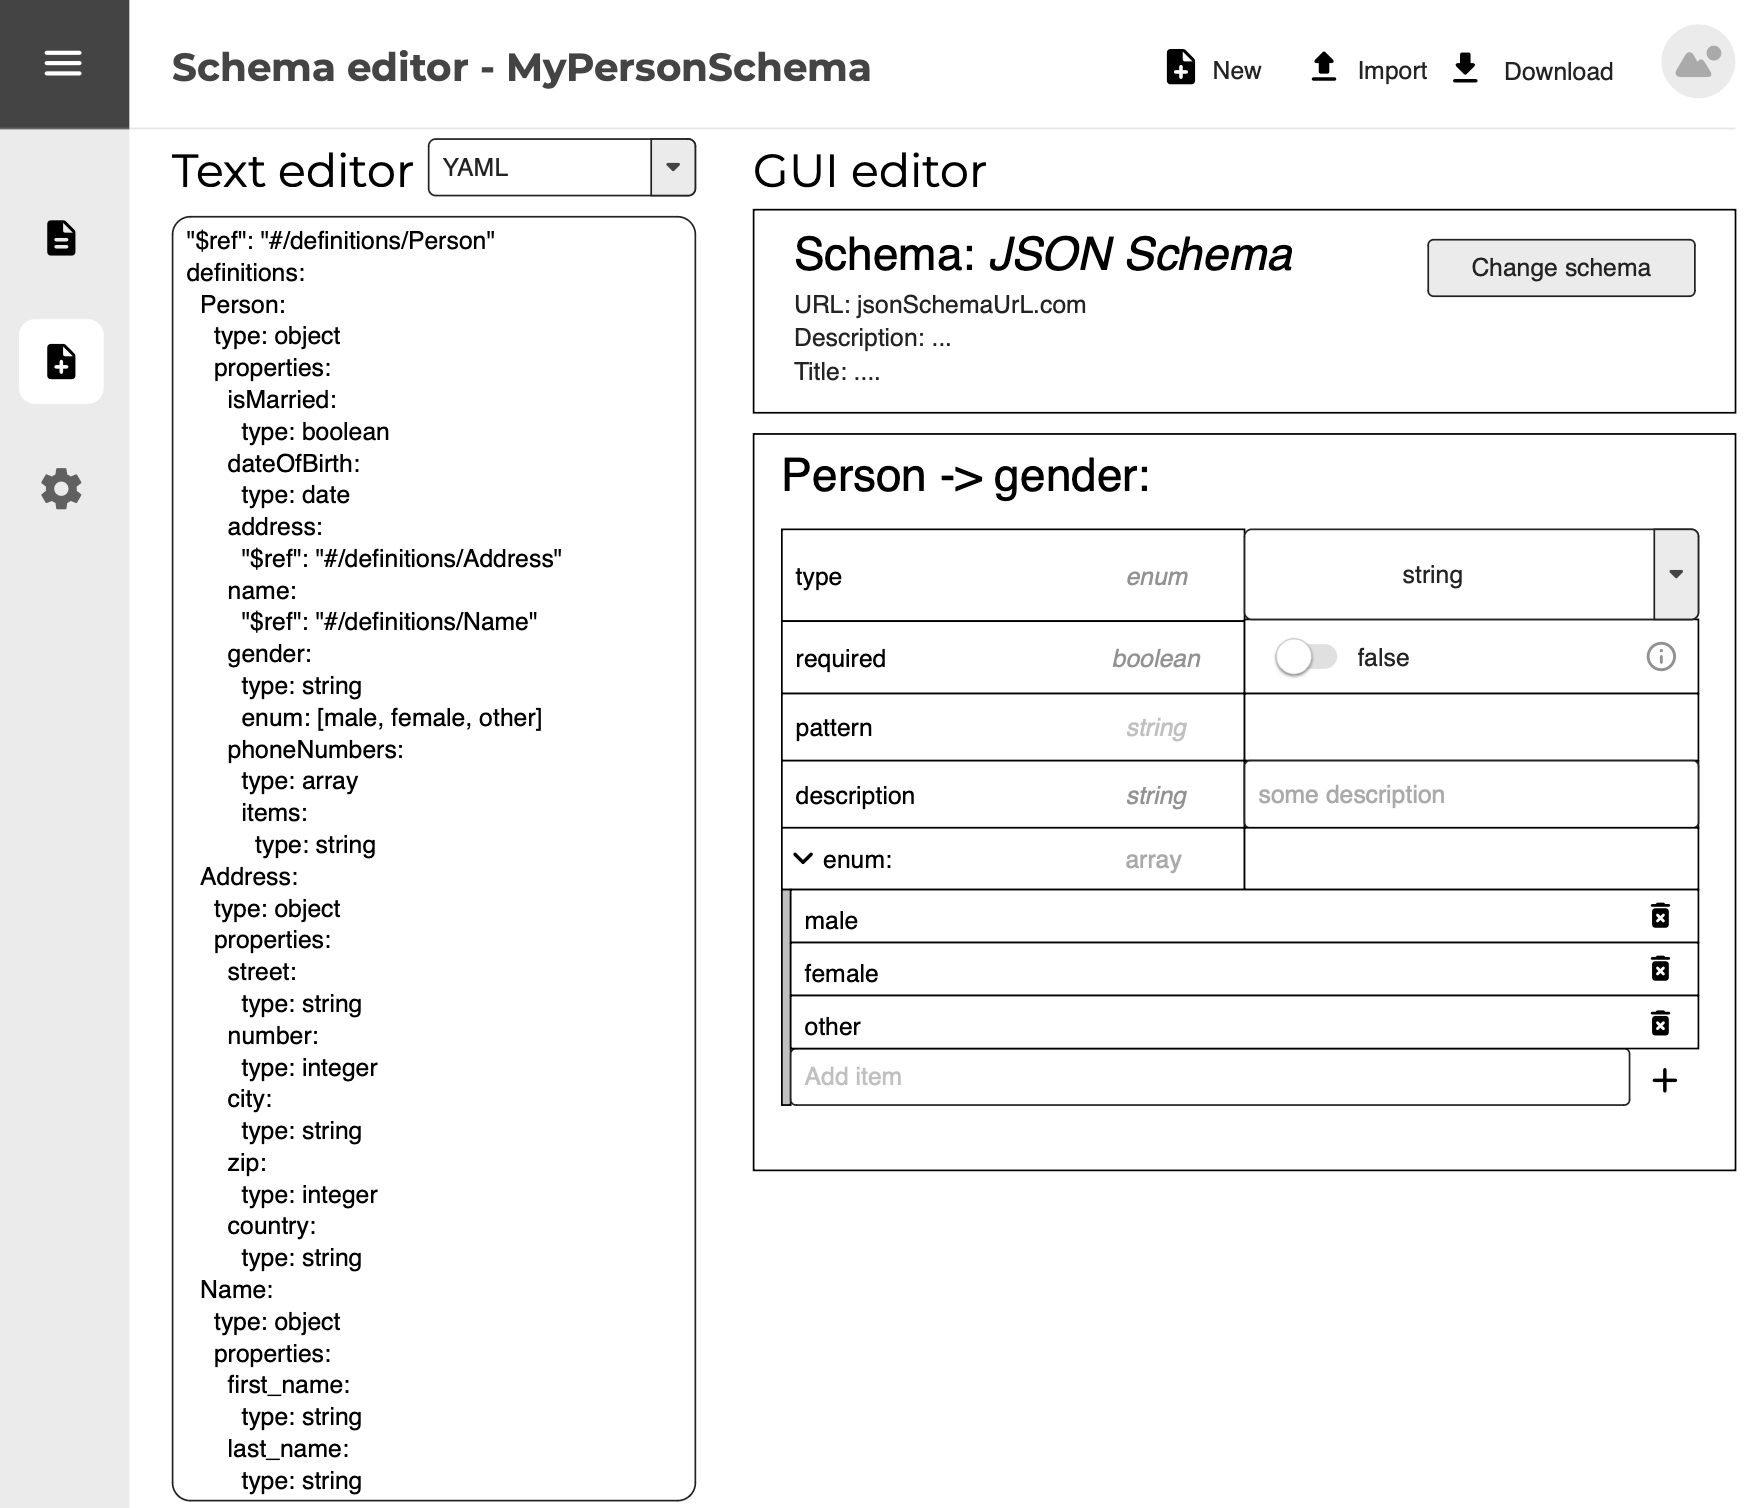
\includegraphics[width=\textwidth]{mockup_gui_schema.png}
\caption{Sketch of the Tool. Workflow: the user creates a schema for their use-case, based on JSON Schema}
\label{mockup_gui_schema}
\end{figure*}

% TODO: add numbered annotations to the screenshot and explain them here
\begin{enumerate}
    \item Blabla this is the menu bar
\end{enumerate}


 

% felix
\subsection{Architecture}
The core of our tool is a single source of truth data store that contains the current user configuration data (as a JavaScript Object). With this data store we can bidirectionally connect what we call "editor panels". An editor panel is a modular component that the user of the tool can access to modify the config data in an indirect way. It might be implemented as a raw text editor, a graphical user interface or any other way in which the data can be presented to the user. All editor panels are independent and do only have access to the data store but not to each other. Every editor panel subscribes to the changes of the data store, so it can be updated accordingly whenever the data in the store is changed. Additionally, every panel has the capabilities of updating the data store themselves, which is done when the user modifies the data in the editor panel. The following example use-cases illustrate the capabilities of this architecture:

\begin{itemize}
    \item Format converter: one panel shows the data in a rich-text editor in JSON format, a second panel shows the data in a rich-text editor in YAML format. Any semantic data change on one panel will cause the same semantic change in the other panel.
    \item Split-Screen Editor: one panel shows the data in a rich-text editor, a second panel shows the data in a GUI. This way the user can have the efficiency of a text editor, but also the assistance of a GUI at the same time. Any semantic data change on one panel will be forwarded to the other panel. The GUI editor panel would require some data schema.
    \item The Split-Screen Editor could be implemented for different data formats, such as YAML, JSON and XML. The architecture allows any data format as long as there exists a mapping from this data format to a JavaScript Object and back.
\end{itemize}

% TODO: Add diagram with store in center in several panels with bidirectional connection of subscribe/update

% felix
\subsubsection{Single Source of Truth Data Store}
this is the core of the tool. The panels can subscribe to this store to receive updates whenever data is changed. Also, panels can trigger changes of the data in the store.
Besides the current configuration data, the store also stores the \textit{path of the currently selected data entry} and the schema that is currently being used.

% felix
\subsubsection{Text Editor Panel}
For the text editor panels, we embed a rich-text editor that already supports syntax highlighting and other useful features. We add validation of whether the text is well-formed according to the JSON/YAML/XML Standard and schema validation. 
The architecture allows for having one text editor panel that supports multiple languages, as well as for having separate text editor panels, one for each language.
The panels subscribe to the data store. Whenever the configuration data is changed in the store, the panels will take the new configuration data JavaScript Object, serialize it into the given language and replace the text in the text editor with the new serialized data.
The action of replacing the text in the text editor will cause formatting and comments to be lost. 
An alternative to replacing the complete text in the text editor, whenever data in the store is changed, would be to only replace the section of the text, which corresponds to the change. This would require 1. identifying which part of the data is affected by the change and 2. understanding of the data within the serialized text in a way that it can be manipulated (e.g. navigating within the hierarchical data structure and changing values of a given path). However, even such deep understanding of the text would wipe out non-default formatting at the sections affected by change. 
We tackle those difficulties in the following way: we accept that user-specific text formatting might be undone by our tool. To allow for different styles of formatting, we will provide the user with global formatting style settings (such as level of indentation or whether in YAML strings should be in quotation marks or not). Whenever the configuration data JavaScript Object is serialized into text, we apply those formatting style settings.
Second, to deal with the loss of comments, we implement a technique that keeps track of any comments in the text and then restores them after the text is replaced.

When the user edits the text in the text editor, the text is deserialized into a JavaScript Object and sent to the data store, which then updates the configuration data object and notifies all other subscribed panels of the change.

% felix
\subsubsection{GUI Assistance Panel}
The GUI assistance panel(s) directly work with the given schema and provide the user with corresponding GUI elements, such as a checkbox for a boolean data structure or a textfield for a string data structure. Additional GUI elements, such as tooltips (showing the description of a data field) are used to support the easier.
The GUI elements are constructed in the following manner: a schema is seen as a hierarchical tree of data field definitions and their corresponding constraints. A data field can either be simple (string, boolean, number, ...) or complex (array or dictionary of data fields). Every schema has a root data field. The GUI element for this root data field is constructed. When constructing the GUI element for a complex data field, this includes constructing the GUI elements for all child data fields too. This way, the whole schema tree is traversed and GUI elements for all entries are constructed.
To avoid overwhelming the user with too many GUI elements, the ones with child elements can be expanded or collapsed by the user and only a limited amount of them is expanded by default.
By design, each of these constructed GUI elements is mapped to their corresponding data field (in other words: to a path in the data structure). The initial values of all GUI elements are taken from the data in the store, by accessing the data at the given paths. Whenever the values in a GUI element are adjusted by the user, the data in the store will be updated with the new values.

In the following, the corresponding GUI elements for the different JSON Schema datatypes and constraints are shown:

\textbf{Boolean}


\textbf{Boolean}

% todo: describe how it works. Then also describe for all the different data types, how we intend to implement the GUI aspect. E.g. for boolean we have checkbox


\section{Methodology}
\subsection{Sections and Subsections}




\subsection{Lists}

\subsubsection*{\bf A plain  unnumbered list}
\begin{list}{}{}
\item{bare\_jrnl.tex}
\item{bare\_conf.tex}
\item{bare\_jrnl\_compsoc.tex}
\item{bare\_conf\_compsoc.tex}
\item{bare\_jrnl\_comsoc.tex}
\end{list}

\subsubsection*{\bf A simple numbered list}
\begin{enumerate}
\item{bare\_jrnl.tex}
\item{bare\_conf.tex}
\item{bare\_jrnl\_compsoc.tex}
\item{bare\_conf\_compsoc.tex}
\item{bare\_jrnl\_comsoc.tex}
\end{enumerate}

\subsubsection*{\bf A simple bulleted list}
\begin{itemize}
\item{bare\_jrnl.tex}
\item{bare\_conf.tex}
\item{bare\_jrnl\_compsoc.tex}
\item{bare\_conf\_compsoc.tex}
\item{bare\_jrnl\_comsoc.tex}
\end{itemize}





\subsection{Figures}
Fig. 1 is an example of a floating figure using the graphicx package.
 Note that $\backslash${\tt{label}} must occur AFTER (or within) $\backslash${\tt{caption}}.
 For figures, $\backslash${\tt{caption}} should occur after the $\backslash${\tt{includegraphics}}.

%\begin{figure}[!t]
%\centering
%\includegraphics[width=2.5in]{fig1}
%\caption{Simulation results for the network.}
%\label{fig_1}
%\end{figure}

Fig. 2(a) and 2(b) is an example of a double column floating figure using two subfigures.
 (The subfig.sty package must be loaded for this to work.)
 The subfigure $\backslash${\tt{label}} commands are set within each subfloat command,
 and the $\backslash${\tt{label}} for the overall figure must come after $\backslash${\tt{caption}}.
 $\backslash${\tt{hfil}} is used as a separator to get equal spacing.
 The combined width of all the parts of the figure should do not exceed the text width or a line break will occur.
%
%\begin{figure*}[!t]
%\centering
%\subfloat[]{\includegraphics[width=2.5in]{fig1}%
%\label{fig_first_case}}
%\hfil
%\subfloat[]{\includegraphics[width=2.5in]{fig1}%
%\label{fig_second_case}}
%\caption{Dae. Ad quatur autat ut porepel itemoles dolor autem fuga. Bus quia con nessunti as remo di quatus non perum que nimus. (a) Case I. (b) Case II.}
%\label{fig_sim}
%\end{figure*}

Note that often IEEE papers with multi-part figures do not place the labels within the image itself (using the optional argument to $\backslash${\tt{subfloat}}[]), but instead will
 reference/describe all of them (a), (b), etc., within the main caption.
 Be aware that for subfig.sty to generate the (a), (b), etc., subfigure
 labels, the optional argument to $\backslash${\tt{subfloat}} must be present. If a
 subcaption is not desired, leave its contents blank,
 e.g.,$\backslash${\tt{subfloat}}[].


 

\section{Tables}
Note that, for IEEE-style tables, the
 $\backslash${\tt{caption}} command should come BEFORE the table. Table captions use title case. Articles (a, an, the), coordinating conjunctions (and, but, for, or, nor), and most short prepositions are lowercase unless they are the first or last word. Table text will default to $\backslash${\tt{footnotesize}} as
 the IEEE normally uses this smaller font for tables.
 The $\backslash${\tt{label}} must come after $\backslash${\tt{caption}} as always.
 
\begin{table}[!t]
\caption{An Example of a Table\label{tab:table1}}
\centering
\begin{tabular}{|c||c|}
\hline
One & Two\\
\hline
Three & Four\\
\hline
\end{tabular}
\end{table}


\section{Conclusion}
The conclusion goes here.


\section*{Acknowledgments}
This should be a simple paragraph before the References to thank those individuals and institutions who have supported your work on this article.



{\appendix[Proof of the Zonklar Equations]
Use $\backslash${\tt{appendix}} if you have a single appendix:
Do not use $\backslash${\tt{section}} anymore after $\backslash${\tt{appendix}}, only $\backslash${\tt{section*}}.
If you have multiple appendixes use $\backslash${\tt{appendices}} then use $\backslash${\tt{section}} to start each appendix.
You must declare a $\backslash${\tt{section}} before using any $\backslash${\tt{subsection}} or using $\backslash${\tt{label}} ($\backslash${\tt{appendices}} by itself
 starts a section numbered zero.)}



%{\appendices
%\section*{Proof of the First Zonklar Equation}
%Appendix one text goes here.
% You can choose not to have a title for an appendix if you want by leaving the argument blank
%\section*{Proof of the Second Zonklar Equation}
%Appendix two text goes here.}



\section{References Section}
You can use a bibliography generated by BibTeX as a .bbl file.
 BibTeX documentation can be easily obtained at:
 http://mirror.ctan.org/biblio/bibtex/contrib/doc/
 The IEEEtran BibTeX style support page is:
 http://www.michaelshell.org/tex/ieeetran/bibtex/

\bibliographystyle{IEEEtran}
 \bibliography{literature}
 % argument is your BibTeX string definitions and bibliography database(s)
%\bibliography{IEEEabrv,../bib/paper}
%
\section{Simple References}
You can manually copy in the resultant .bbl file and set second argument of $\backslash${\tt{begin}} to the number of references
 (used to reserve space for the reference number labels box).

%\begin{thebibliography}{1}
%\bibliographystyle{IEEEtran}


%\end{thebibliography}


\newpage

\section{Biography Section}
If you have an EPS/PDF photo (graphicx package needed), extra braces are
 needed around the contents of the optional argument to biography to prevent
 the LaTeX parser from getting confused when it sees the complicated
 $\backslash${\tt{includegraphics}} command within an optional argument. (You can create
 your own custom macro containing the $\backslash${\tt{includegraphics}} command to make things
 simpler here.)
 
\vspace{11pt}

\bf{If you include a photo:}\vspace{-33pt}
%\begin{IEEEbiography}%[{\includegraphics[width=1in,height=1.25in,clip,keepaspectratio]{fig1}}]{Michael %Shell}
%Use $\backslash${\tt{begin\{IEEEbiography\}}} and then for the 1st argument use %$\backslash${\tt{includegraphics}} to declare and link the author photo.
%Use the author name as the 3rd argument followed by the biography text.
%\end{IEEEbiography}

\vspace{11pt}

\bf{If you will not include a photo:}\vspace{-33pt}
\begin{IEEEbiographynophoto}{John Doe}
Use $\backslash${\tt{begin\{IEEEbiographynophoto\}}} and the author name as the argument followed by the biography text.
\end{IEEEbiographynophoto}




\vfill

\end{document}


